% !TeX spellcheck = en_EN-English

\section{Embedding of patient}
\label{embedding}

First of sub-tasks for prediction of patient future costs is to embed each patient record into numerical vector that would be understandable for neural network. For each record of a patient we embed four information. First and easy to implement is a timestamp which is computed using numerical and date values, then there three more tricky information and those are diagnosis, medical procedure and prescribed drug. 

\subsection{Timestamp}

Attribute what we call timestamp of patients record can more precisely described as approximation of patients age at the moment of either medical procedure or drug prescription. This timestamp is computed using two of available information and those are age of patient in years and date of record. Computation for single patient is done like this: we found first record of patient, meaning record with earliest date, and we take age in years of that patient in that moment and set it as a timestamp, for each next record we that age from first record and add difference between first record and currently processed one conversed to fraction of years. This way timestamp contains approximation of age of patient while also containing information about order of records and comparative timeframe between each two records.

\subsection{Diagnosis embedding}

Base diagnose information we embed was ICD-10-CM code of disease.ICD-10-CM stands for "International Classification of Diseases, Tenth Revision, Clinical Modification" and is used to code and classify medical diagnoses \cite{cdcICD10CM} most precisely version of this code that is used in Slovakia and is better known by the acronym MKCH-10-SK (Medzinárodná klasifikácia chorôb) \cite{ncziMKCH}.\\

\begin{figure}[!h]
	\centering
	
	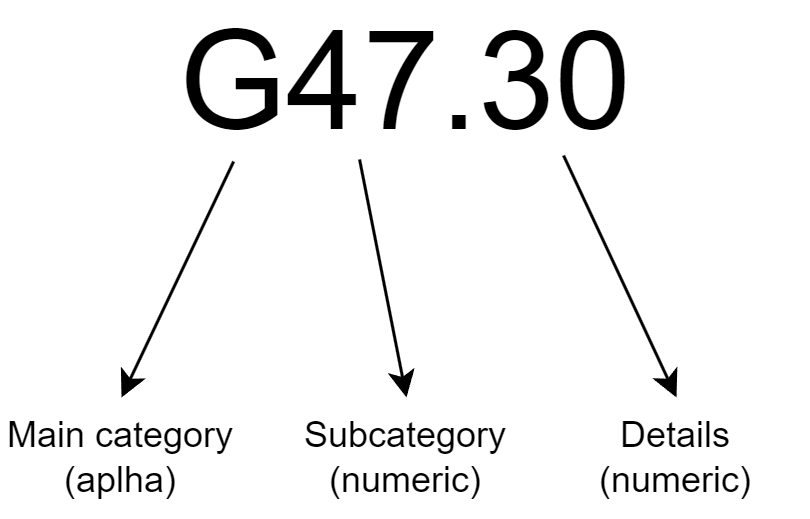
\includegraphics[width=0.8\textwidth]{images/ICD-10-CM.png}
	
	\caption{Structure of MKCH-10 code}
	\label{fig:icd-10-cm}
\end{figure}

This code consist of three parts as shown on image \ref{fig:icd-10-cm}. First part is one letter that encodes main categories of diseases also known as chapter, for example codes starting with G are diseases of the nervous system. 
After that there is two numeric characters that further specify subcategory of disease such as codes from G40 to G47 which are episodic and paroxysmal disorders and specifically G47 are sleep disorders. 
We can see that episodic and paroxysmal disorders are only up to G47, meaning that theoretically there can exist subgroups G48 and G49 which have 4 in second position but does not belong to same G4 subcategory as G40 or G47 \label{mkch_subdiv}. Thankfully this is not the case and in cases like this when higher lower subcategory (like G4) does not have 10 lower level subcategories (like G47) these subcategories does not exist at all and in case it have more than 10 lower level subcategories it gets multiple consecutive high level subcategories, for example disorders of other endocrine glands spans from E20 to E35. 
Then code contains dot after which there are characters that further describe details of disease such as etiology, anatomic site and severity. Official documentation of ICD-10-CM codes stands that codes can be up to 7 characters long meaning that after first three characters specifying category there can be up to 4 alphanumeric to further specify the disease \b{CITE}, however Slovak version MKCH-10 codes contains at most two numeric characters to specify disease \b{cite} and these details are organized in a way where the first position conveys higher-level information than the second, for example G47.3 is sleep apnea and G47.30 is primary central sleep apnea.
\\

To embed this code we firstly split it into it's three parts and embed each part separately. After that we concatenated embedding of each part to get final embedding of disease.
To embed main category we generated vector containing random numbers from interval [-0.5, 0.5] using uniform distribution for each letter of English alphabet (all main categories). We used random vectors in order to have relatively similar distance between any two main categories since there are no particular relationships between these categories, we were thinking also about using one-hot encoding which would make distance between each two categories perfectly same but we didn't do it since it would have restricted length of vector. 
In embedding second part which is subcategory we used different approach, where to each number between 00 and 99 (all possible values of this part) we assign linearly number between -0.5 and 0.5, meaning subcategory 00 would get -0.5 category 50 would get 0 and category 99 would get 0.5, we choose these boundaries in order to match mean and variance of of numbers generated for main category. This assigned number was then repeated multiple times to create vector. This approach has advantages and disadvantages. Advantage is that we can be sure that closely related disease subgroups like G46 and G47 would get close embedding since their subgroup codes are close on number line. However there are also two disadvantages, first is that G49 and G50 would be similarly close as G46 and G47, but thankfully in a most cases either X9 code doesn't exist at all, creating a gap, or if X9 code exist it belong to category that go past X on as higher level subgroup. Another disadvantage is that distance between two higher level subgroups can vary quite dramatically even though in reality there might not be reason for that difference in distance. For example, using this approach higher level subgroup G40-G47 is much closer to subgroup G50-G59 than to G80-G83.
Finally to embed details we decided to use same approach as for subgroups since these codes work similarly, only difference was that not all codes had second level details, in such cases we add 5 as a proxy in order to minimize average distance from all potential codes with same first level details code that contain second level detail information while also maximizing average distance to different first level detail codes.
Final after embedding each part final embedding is created as their concatenation, to encode importance of each part in final embedding we gave them different lengths, this works thanks to the fact that each value in each of vector have same mean and same variance. Main category, the most important part, got vector of length 26, subcategory part got length 9 and finally details got length 3.
Showcase of resulting embedding can be seen on image \ref{fig:diag_emb_show} where each part is highlighted by different color and all values are rounded to two decimal.
In order to confirm that our embedding has desired properties we computed similarity of embedding of multiple codes. As similarity function we choose simple multiplicative inverse of Euclidean distance. In table \ref{tab:diag_emb_show} we can see results. Highest similarity was between codes G47.30 and G40.09 which is expected since they belong to same main category and very close subcategory, second highest was between H40.09 and H18.80 which are only other combination that belong to same main category, this confirms that main category has biggest impact since this similarity is significantly higher than that between G40.09 and H40.09 which differ only main category.

\begin{figure}[!h]
	\centering
	
	% TODO image needs update after change of lengths of each embeddings
	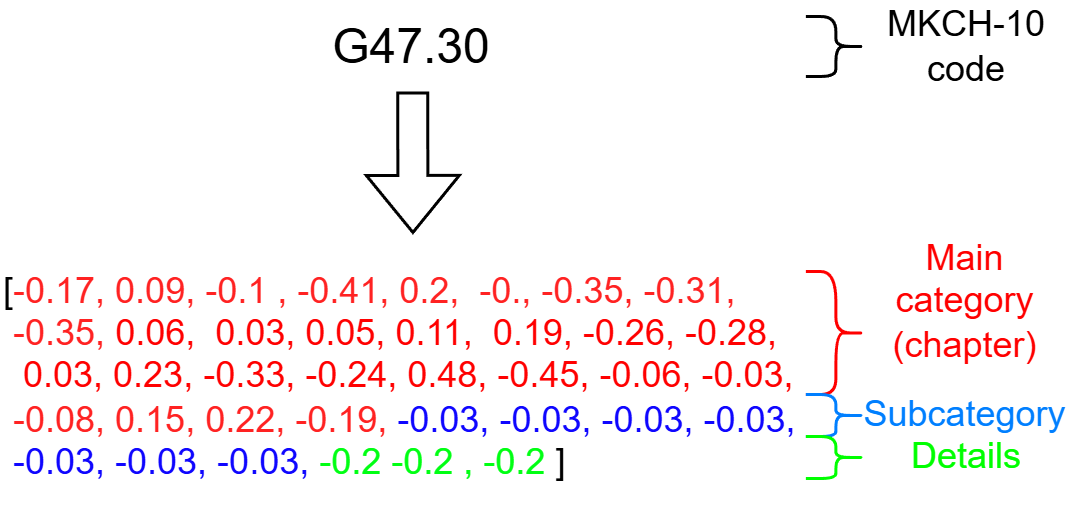
\includegraphics[width=0.8\textwidth]{images/diagnosis_embed_showcase.png} 
	
	\caption{Showcase of resulting embedding of specific diagnosis (rounded to two decimal places)}
	\label{fig:diag_emb_show}
\end{figure} 


\begin{table}[!h]
	\centering
	\begin{tabular}{|l|l|l|}
		\hline
		Code A & Code B & Similarity \\ \hline
		G47.30 & G40.09 & 2.77       \\ \hline
		G47.30 & H40.09 & 0.53       \\ \hline
		G47.30 & H18.80 & 0.46       \\ \hline
		G40.09 & H40.09 & 0.54       \\ \hline
		G40.09 & H18.80 & 0.45       \\ \hline
		H40.09 & H18.80 & 0.84       \\ \hline
	\end{tabular}
	\caption{Similarities of embedding of multiple chosen MKCH-10 codes}
	\label{tab:diag_emb_show}
\end{table}  

\subsection{Drug embedding}

Similarly to diagnosis, to embed drug information we embed international code associated to these drug. In case of drugs it was Anatomical Therapeutic Chemical classification system also known under abbreviation ATC. In a same way as MKCH-10 code this code can be split into multiple parts where each next part contains finer information. It contains of 5 parts or levels. First level encodes main anatomical or pharmacological groups. There are fourteen such groups, encoded by single letter, which are shown in the figure \ref{fig:atc_l1}. Then second level encodes pharmacological or therapeutic subgroup using two digit number, after that there two levels that further specify pharmacological, therapeutic or even chemical subgroup, these two levels are both encoded using single letter each. Final fifth encoded with two digit number contains information about specific chemical substance inside drug.

\begin{figure}[!h]
	\centering
	
	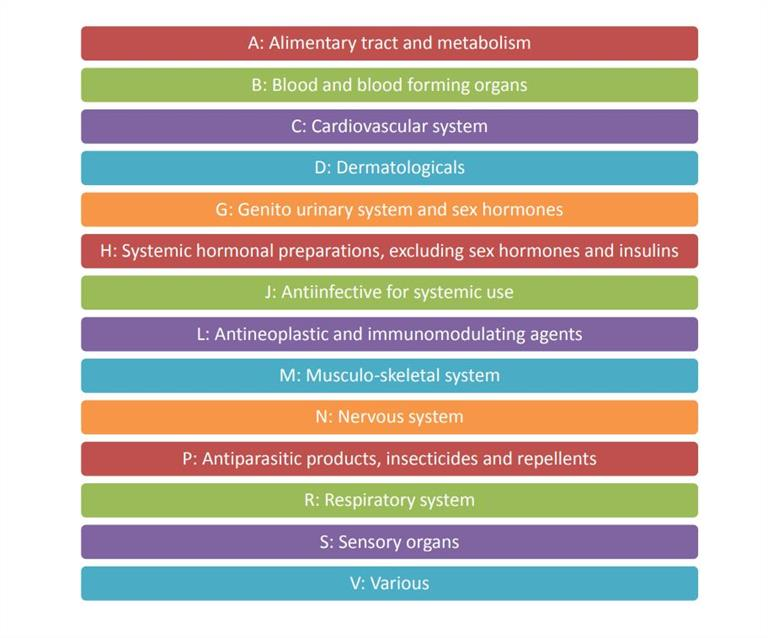
\includegraphics[width=0.8\textwidth]{images/atc_l1_classification_who.jpg}
	
	\caption{Fourteen main anatomical or pharmacological groups and their corresponding first level ATC code \cite{atc_who}}
	\label{fig:atc_l1}
\end{figure}

Embedding was done in very similar way as in diagnosis embedding, meaning each level was embedded separately and final embedding was done as concatenations of them. In this case each level was embed using random vector from uniform distribution with interval [-0.5, 0.5]. We used random vectors for each level since none of levels contains any internal sub-groupings similar to subgroups of diagnosis (see \ref{mkch_subdiv} subgroup codes). To encode importance of levels we again used lengths of random vectors, where with higher level vectors shortens. Lengths of vectors for each level can be seen in \ref{tab:drug_lev_len}. So total length of embedding is same as embedding for diagnosis.In case code is incomplete, meaning it's missing higher levels, missing part is substituted with zeros which we consider neutral elements.
\\

\begin{table}[!h]
	\centering
	\begin{tabular}{|l|l|}
		\hline
		Level  & Length \\ \hline
		1 & 20 \\ \hline
		2 & 10 \\ \hline
		3 & 5 \\ \hline
		4 & 2 \\ \hline
		5 & 1 \\ \hline
	\end{tabular}
	\caption{Lengths of random vectors assigned to each information level of ATC code}
	\label{tab:drug_lev_len}
\end{table}  

With this embedding we should get codes whose similarity is more dependent on whether lower more important levels match than higher ones. To confirm this we do similar check as we did with diagnosis code and compute similarity of four chosen ATC codes and see if our theory holds. To compute similarity we again use multiplicative inverse of Euclidean distance. We choose C01EB15, C01CA04, C10AA07 and J01CA04, we would expect first two to be most similar since they match on first levels, than first two compared to third should have slightly lower similarity since they match on only first level and finally we expect that all three would be least similar to fourth one since first level is different, even though that second and forth match on all other levels.  We can see results in table \ref{tab:drug_emb_show}. We can see that results met our expectation with highest similarity between first two and lowest between any of first three and fourth, even in case of second and forth that match on all other levels except first.

\begin{table}[!h]
	\centering
	\begin{tabular}{|l|l|l|}
		\hline
		Code A & Code B & Similarity \\ \hline
		C01EB15 & C01CA04 & 1.24      \\ \hline
		C01EB15 & C10AA07 & 0.54       \\ \hline
		C01EB15 & J01CA04 & 0.45       \\ \hline
		C01CA04 & C10AA07 & 0.64       \\ \hline
		C01CA04 & J01CA04 & 0.48       \\ \hline
		C10AA07 & J01CA04 & 0.38       \\ \hline
	\end{tabular}
	\caption{Similarities of embedding of multiple chosen ATC codes}
	\label{tab:drug_emb_show}
\end{table}  

\subsection{Medical procedure embedding}

Final and most difficult part to embed was medical procedures. In this case there is no structured code that can be used and is implemented in Slovak healthcare systems. So what we have done is to embed description of the procedures. For that we used large language model (LLM) trained on multiple languages including Slovak. Dimensionality of resulting embedding was then reduced using PCA, to get rid of dimensions with small variance meaning they encode small amount of information. 
\\

For LLM we choose language-agnostic BERT sentence embedding also known under abbreviation LaBSE. It's a model developed by Goggle to encode text into high dimensional vectors. This model was trained 109 languages including Slovak. Main goal of this model is to generate similar representation to pairs of sentences which have same meaning and are only translations in two different language \cite{labse_kaggle}. This approach should produce better results compared to standard text embedding models trained solely on Slovak language, since LaBSE model is during training comparing embedding not only to similar sentences in Slovak language but also their translation in other which could mitigate a relatively small amount of Slovak language data compared to other more commonly used languages. Additionally this model could know domain specific words in our case medical terms which are left in foreign language and would most likely not be found in Slovak only corpus. To confirm this expectation, we compare results to Word2Vec model trained on purely Slovak language using corpus containing 110 million words \cite{word2vec}. As a way of comparison we choose to  firstly group embedding into categories using K-nearest neighbors algorithm (KNN), and visually asses whether description in resulting categories show any resemblance or whether they seem random. 
\\
Architecture of LaBSE model consist of 4 parts \cite{labse_hug}:

\begin{enumerate}
	\item Encoder-only transformer (BERT model)
	\item Pooling layer
	\item Dense layer
	\item Normalization layer
\end{enumerate}

\subsubsection{Encoder-only transformer (BERT model)}
\label{emb:trans}

First and most important part of LaBSE model is transformer, which is a deep learning architecture. More specifically LaBSE uses BERT so bidirectional encoder representations from transformers model which is encoder-only transformer architecture meaning this model does not contain decoder found in standard transformer which is usually used for prediction, because of this BERT model is focused in extracting contextual information from input text. Architecture of standard BERT model looks like this: 
\\

\begin{enumerate}
	\item Tokenizer layer
	\item Embedding layer
	\item Encoder
	\item Task layer
\end{enumerate}

First layer is tokenizer, this layer takes input text split it into tokens which in case of BERT model is called PieceWise tokenizer which split text into subwords so something close to syllables. PieceWise tokenizer has advantage compared to different tokenizers that use either words or characters. Compared to character wise tokenizing, subwords contain more information than characters, and compared to word tokenizer is that there a lot less subwords than words and are more similar across multiple languages, creating much smaller vocabulary which is especially important for multilingual models. After split this layer assign integer number to each unique token, LaBSE model vocabulary distinguishes around 500 000 different tokens.
\\

After that comes embedding layer which assign real number vector to each token, more specifically BERT model compute three different embeddings and add them together and normalize result to get final one. First is token type embedding, which is basic embedding where each token in vocabulary is assigned it's unique embedding. Second is positional embedding, as name suggest this embedding contain information about where in the sequence token is found giving additional information. Third and final embedding is segment type, which encodes information about to which segment, usually sentence token belong, important for embedding input text consisting of multiple sentences.
\\

Third and most important layer is encoding. This is the layer in which contextual information are mined from the text. This consist of multiple attention block stacked one after the other. In case of BERT used in LaBSE there are 12 such blocks. Each attention block consist of two parts, multi-headed self-attention layer and multi-layered feed-forward neural network. 
\\

Each head of self-attention layer takes a input set of embeddings and to compute new set of embeddings which should encode not only original information but also information about relationship between original ones, in other words it encodes effect of tokens onto each other. To do that it compute for each input embedding three vectors usually called key, query and value by multiplying input embedding with three matrices which values are learned during training. After that to get new embedding query vector is multiplied with matrix created from key vectors so resulting vector is vector of dot product of single query and all keys, this vector then goes through softmax function to normalize result. In some transformer models before softmax this vector get masked. Masking is done by setting values where key vector belongs to later embedding than query to minus infinity, this way after softmax this values become zeros. This is done so that later embedding does not affect previous ones. It's mostly useful in models trained to predict next token in order for model to learn to predict only based on tokens from past on not future. However in case of model like BERT where emphasis is on extracting as much information from input text masking is not done. Final step to get new embedding is to multiply vector we got after applying softmax with matrix composed of value vector to get linear combination of value vectors. This resulting vector is new embedding. This is done for all query vectors. List list resulting vectors is output embedding of attention head. Since this model use multi-headed attention more specifically in case of LaBSE 12-headed attention, this process is simultaneously independently done 12 times and results of each head are than concatenated into final result of attention. By using multiple head we expect that each head can extract different information from input and final concatenation give us result that contains all extracted information.    
\\

This concatenation of new embeddings goes than into multi-layered feed-forward neural network, which consist of multiple fully connected or in other words dense layers with activation layers in between them.
\\

Result goes to next attention block and process is repeated again. Result of final attention block then goes to last part which is task layer, this layer can be viewed as simple decoder that map resulting embeddings back into token space. Based on this results is then model pre-trained. Training process of BERT model usually consist of two tasks on which are model trained at the same time. First is masked language modeling (MLM) where 15\% of input tokens are masked meaning either replaced by mask placeholder or by random different token, after that masked input goes into model, then from resulting tokens are taken those on position of masked tokens in input and are compared to correct token before masking which creates error that is back-propagated through model updating it's parameters \cite{bert_pretr_1}. Other task usually used is called next sentence prediction (NSP), in this task model gets input which start with special classify token and after that two spans of texts separated by special separator token. Task of model is to say whether these two spans of text can appear one after another or more precisely whether they appeared one after another in training corpus and put this information into first token of result encoded by two special tokens either "is next" or "not next" token and similarly difference between expected and resulting first token create error that back-propagates through model \cite{bert_pretr_2}. However in some BERT-based model like LaBSE second task is replaced with translation language modeling (TLM), this task is extention of MLM in which model gets two concatenated sentence instead of one and where the second sentence is translation of the first in another language, rest of the task is than same as in MLM, so whole input gets masked and model is tasked to predict masked tokens \cite{bert_pretr_3}. Task layer is used primarly in only during pre-training and is omitted when model is used for different task as many use-cases does not need tokens in results but use embeddings from encoding layer as form of text encoding which is that further used in task specific layers on which then model is fine-tuned.

\subsubsection{Pooling layer}

After BERT model returns embeddings of all input tokes, these then needs to be aggregated into single vector which corresponds to embedding of whole input. This aggregation is done using pooling layer. In case of LaBSE this pooling is done simply by taking embedding of first token which is an embedding of special classify token added to beginning of BERT input.    

\subsubsection{Dense layer}

Next layer is standard feed forward dense layer with use hyperbolic tangent activation function. Number of input and output neurons is same, and additional bias neuron is used.

\subsubsection{Normalization layer}

Final layer is normalization which task is only to normalize resulting vector, so divide vector by number in order to have final vector with $L_2$ norm equal one.
\\

After we embed each description of procedure using LaBSE model, we get 768 dimensional vectors assigned to them. As this dimensionality is relatively high, especially when we consider that descriptions of procedures used limited primarily medical vocabulary, we decided to use dimension reduction technique in order to remove dimensions which are least informative and contribute mostly noise. We used principal component analysis (PCA).
\\

Finally we create record embedding by concatenating all four parts. Since we have two separate datasets, one for prescribed drugs and one for medical procedures, we always have only three out of four information available for each record, since timestamp and diagnosis are always available, we substitute missing part with vector of zeros with appropriate length which is most neutral embedding since we centered both medical procedure and drug prescription embedding around zero.
